\section{Nota Teórica}
\subsection{Características Generales}
El microcontrolador ATtiny4313 de Atmel es una unidad de 8 bits diseñada para ofrecer un alto rendimiento. Gracias a su arquitectura RISC avanzada, el dispositivo ofrece una programación en sistema altamente flexible. Además, cuenta con una amplia gama de periféricos incorporados y es notable por sus múltiples opciones para el bajo consumo de energía. Todas las características técnicas descritas en esta sección se basan en la hoja de datos oficial del microcontrolador ATtiny4313 \cite{Atmel2011}.

\subsection{Arquitectura RISC Avanzada}
\begin{itemize}
    \item 120 instrucciones potentes, la mayoría con ejecución de un solo ciclo de reloj
    \item 32 x 8 registros de trabajo de propósito general
    \item Operación completamente estática
    \item Hasta 20 MIPS de rendimiento a 20 MHz
\end{itemize}

\subsection{Memorias de Programa y Datos No Volátiles}
\begin{itemize}
    \item 2/4K Bytes de Flash programable en el sistema
    \item Durabilidad de 10,000 ciclos de escritura/borrado
    \item 128/256 Bytes de EEPROM programable en el sistema
    \item Durabilidad: 100,000 ciclos de escritura/borrado
    \item 128/256 Bytes de SRAM interna
\end{itemize}

\subsection{Características Periféricas}
\begin{itemize}
    \item Un contador de temporizador de 8 bits con preescalador y modo de comparación separados
    \item Un contador de temporizador de 16 bits con preescalador, modos de comparación y captura separados
    \item Cuatro canales PWM
    \item Comparador analógico en chip
    \item Temporizador de vigilancia programable con oscilador en chip
    \item USI: Interfaz Serial Universal
    \item USART dúplex completo
\end{itemize}

\subsection{Características Especiales del Microcontrolador}
\begin{itemize}
    \item debugWIRE para depuración en chip
    \item Programable en el sistema a través del puerto SPI
    \item Fuentes de interrupción externas e internas
    \item Modos de bajo consumo: inactivo, apagado y en espera
\end{itemize}
\subsection{I/O, Voltaje de Operación y Otras Especificaciones}
\begin{itemize}
    \item 18 líneas I/O programables
    \item Paquetes de 20 pines PDIP, SOIC, y 20-pads MLF/VQFN
    \item Voltaje de operación entre 1.8 – 5.5V
    \item Grados de velocidad:
    \begin{itemize}
        \item 0 – 4 MHz a 1.8 – 5.5V
        \item 0 – 10 MHz a 2.7 – 5.5V
        \item 0 – 20 MHz a 4.5 – 5.5V
    \end{itemize}
    \item Rango de temperatura industrial: -40°C a +85°C
    \item Bajo consumo de energía:
    \begin{itemize}
        \item Modo Activo: 190 $\mu$A a 1.8V y 1MHz
        \item Modo Inactivo: 24 $\mu$A a 1.8V y 1MHz
        \item Modo de Apagado: 0.1 $\mu$A a 1.8V y +25°C
    \end{itemize}
\end{itemize}
\subsection{Diagrama de Pines}
A continuación se presenta el diagrama de pines del ATtiny4313:

\begin{figure}[H]
    \centering
    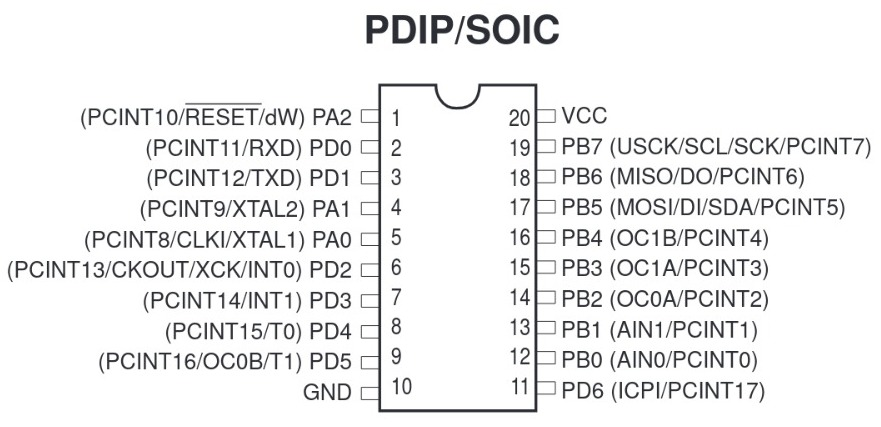
\includegraphics[scale=0.35]{images/Diagrama_pines.jpeg}
    \caption{Diagrama de pines\cite{Atmel2011}.}
    \label{fig:diagrama_pines}
\end{figure}

Para el presente laboratorio, se utilizaron los siguientes puertos: PB0, PB1, PB2, PB3, y PD2. 
\subsection*{Port B (PB7..PB0)}
Port B es un puerto de E/S bidireccional de 8 bits con resistencias pull-up internas que pueden ser seleccionadas para cada bit. Los búferes de salida de Port B presentan características de manejo simétricas, con alta capacidad tanto para hundir como para suministrar corriente. Cuando se utilizan como entradas, los pines de Port B que están externamente tirados a bajo generarán corriente si las resistencias pull-up están activadas. Los pines de Port B entran en estado de alta impedancia cuando se activa una condición de reinicio, incluso si el reloj no está en funcionamiento \cite{Atmel2011}.

\subsection*{Port D (PD6..PD0)}
Similar a Port B, Port D es un puerto de E/S bidireccional de 7 bits con resistencias pull-up internas seleccionables para cada bit. Los búferes de salida de Port D también tienen características simétricas de manejo de corriente. Al igual que con Port B, los pines de Port D que están externamente tirados a bajo generarán corriente si se activan las resistencias pull-up. Los pines de Port D también se ponen en estado de alta impedancia durante una condición de reinicio, incluso si el reloj no está funcionamiento \cite{Atmel2011}.

\begin{figure}[H]
    \centering
    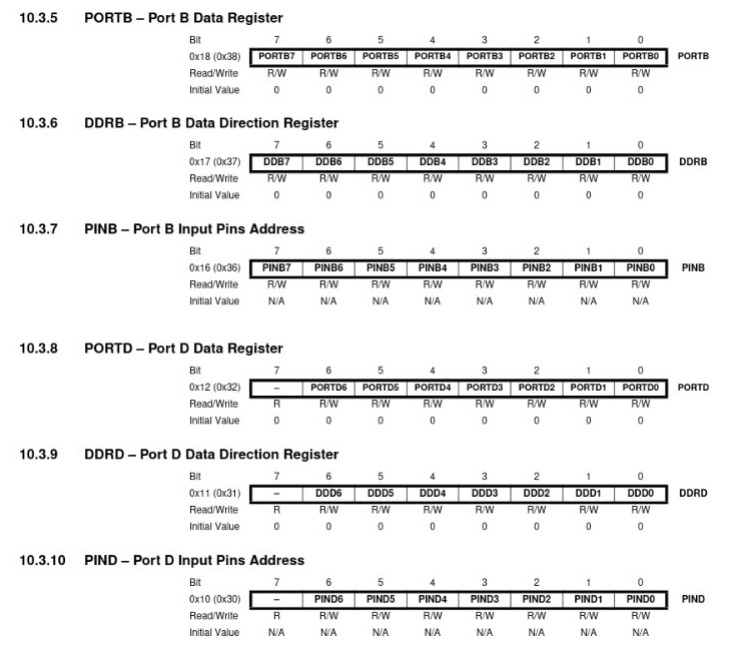
\includegraphics[scale=0.45]{images/puerto.jpeg}
    \caption{Descripción de pines\cite{Atmel2011}.}
    \label{fig:descripcion_pines}
\end{figure}

\subsection{Diagrama de bloques}
A continuación se presenta el diagrama de bloques del ATtiny4313:
\begin{figure}[H]
    \centering
    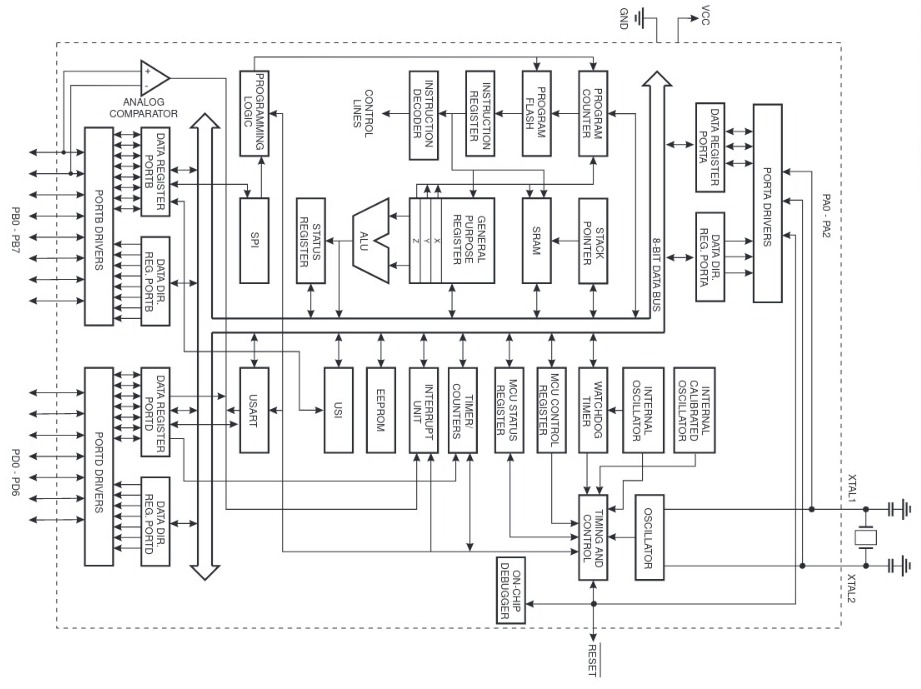
\includegraphics[angle=90, scale=0.4]{images/Diagra_bloques.jpeg}
    \caption{Diagrama de bloques \cite{Atmel2011}.}
    \label{fig:enter-label}
\end{figure}

\subsection{Interrupciones}

Las interrupciones son fundamentales para el funcionamiento eficiente de un microcontrolador. Cuando se activa una interrupción, la ejecución normal del programa se detiene temporalmente. El estado actual del programa, incluidas las variables y el contador de programa, se guarda en un bloque de memoria especial. Luego, el microcontrolador busca en este bloque para encontrar la Rutina de Servicio de Interrupción (ISR) correspondiente que necesita ser ejecutada \cite{Alley2011}.

Existen cuatro componentes clave en el mecanismo de interrupción:

\begin{enumerate}
  \item \textbf{Banderas de Interrupción:} Indican si ha ocurrido un evento de interrupción.
  \item \textbf{Bits de Habilitación de Interrupción:} Determinan si una interrupción específica será atendida automáticamente por el hardware.
  \item \textbf{Habilitación Global de Interrupciones:} Permite o impide que ocurran interrupciones en el sistema.
  \item \textbf{Rutina de Servicio de Interrupción (ISR):} Es el conjunto de instrucciones que se ejecuta cuando se produce una interrupción \cite{Alley2011}.
\end{enumerate}

La ejecución eficiente de las ISRs es crucial para el rendimiento del sistema, ya que evita pérdida de datos o comportamientos inesperados. Estas rutinas son responsables de guardar y restaurar el contexto del programa, permitiendo que el microcontrolador continúe su ejecución donde la dejó \cite{Alley2011}.


\subsection{Interrupciones Externas}
Las interrupciones externas son mecanismos que permiten a un microcontrolador detectar un cambio de estado en alguna de sus terminales de entrada, evitando así la necesidad de un sondeo continuo. Estas son especialmente útiles para monitorear estados de interruptores, botones, o sensores con salida a relevador. \cite{interrupciones}


\subsection{Configuración de las interrupciones}
Las interrupciones externas pueden configurarse para detectar un nivel bajo de voltaje o una transición en el flanco de subida o bajada. Sin embargo, la interrupción INT2 sólo puede activarse por flancos. Importante resaltar que estas interrupciones pueden generarse incluso cuando sus terminales respectivas son configuradas como salidas.

Las transiciones en INT0/INT1 requieren de una señal de reloj (clkI/O) para generar una interrupción. Esta señal de reloj es anulada en la mayoría de los modos de bajo consumo. Por otro lado, un nivel bajo en INT0/INT1 y las transiciones en INT2 no requieren de una señal de reloj, siendo eventos asíncronos y adecuados para despertar al microcontrolador en cualquier modo de reposo.\cite{interrupciones}
\begin{figure}[H]
    \centering
    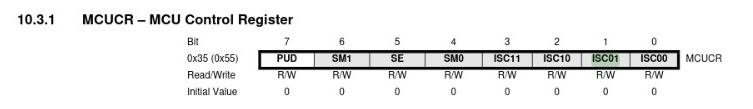
\includegraphics[scale=0.5]{images/MCUCR.jpeg}
    \caption{Configuración del MCUCR\cite{Atmel2011}.}
    \label{fig:enter-label}
\end{figure}
\begin{figure}[H]
    \centering
    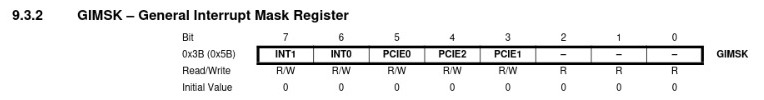
\includegraphics[scale=0.5]{images/GIMSK.jpeg}
    \caption{Configuración del GIMSK\cite{Atmel2011}.}
    \label{fig:enter-label}
\end{figure}
\begin{figure}[H]
    \centering
    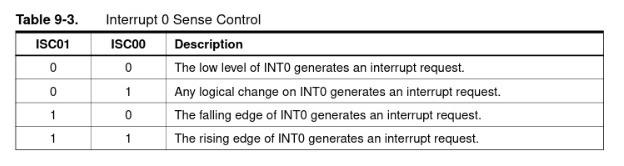
\includegraphics[scale=0.5]{images/int0.jpeg}
    \caption{Configuración del INT0\cite{Atmel2011}.}
    \label{fig:enter-label}
\end{figure}
\subsubsection{Configuraciones Específicas}

\paragraph{NT0: External Interrupt Request 0 Enable}
Cuando este bit y el bit I en el Registro de Estado (SREG) están activados, se habilita la interrupción externa en el pin INT0. Los bits de Control de Sentido de Interrupción (ISC01 y ISC00) en el Registro de Control de Interrupción Externa A (EICRA) determinan si la interrupción se activa en los bordes ascendentes y/o descendentes del pin INT0.

\paragraph{PUD: Pull-up Disable}
Al escribir un ``uno'' en este bit, se desactivan las resistencias \textit{pull-up} en los puertos de E/S.

\paragraph{ISC01, ISC00: Interrupt Sense Control 0 Bit 1 and Bit 0}
La Interrupción Externa 0 se activa por el pin externo INT0 si la bandera I del SREG y la máscara de interrupción correspondiente están establecidas.

\paragraph{Duración de la Señal para Interrupción}
Si se selecciona una interrupción de borde o de conmutación, los pulsos que duran más de un período de reloj generarán una interrupción. Los pulsos más cortos no garantizan la generación de una interrupción.

\subsection{Temporización en Microcontroladores ATMega}

\subsubsection{Importancia de la Temporización Precisa}

Mantener un tiempo preciso es crucial, especialmente en tareas que requieren mediciones exactas o en sistemas de navegación. Los temporizadores internos del microcontrolador permiten una gestión del tiempo altamente precisa, esencial para el control eficaz del sistema \cite{Alley2011}.

\subsubsection{Tipos de Temporizadores}

\paragraph{Temporizadores Internos}
Los microcontroladores ATMega8 y ATMega16 cuentan con temporizadores 0 y 1 que pueden funcionar como contadores de eventos externos.

\paragraph{Temporizadores Externos}
Están diseñados para funcionar con señales externas a través de los pines T0 y T1. Además, el temporizador 2 puede operar con un oscilador externo de 32.768 KHz.

\subsubsection{Modos de Operación}

\begin{itemize}
    \item \textbf{Modo 0:} Operación básica con eventos de desbordamiento.
    \item \textbf{Modos 1 y 3:} Utilizados para la generación de señales PWM.
    \item \textbf{Modo 2:} Permite limpiar el registro del temporizador en coincidencias específicas \cite{interrupciones}.
\end{itemize}

\subsubsection{Registros Importantes}
El temporizador 1 utiliza registros de 16 bits como TCNT1, OCR1A, OCR1B e ICR1 que son esenciales para su funcionamiento. Los registros TCCR1A y TCCR1B controlan el comportamiento del temporizador.
\begin{figure}[H]
    \centering
    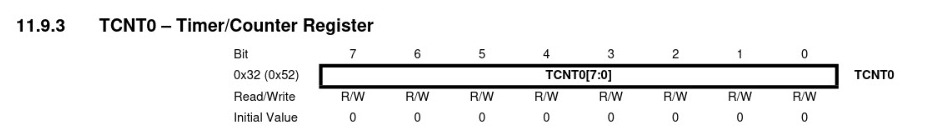
\includegraphics[scale=0.5]{images/TCNT0.jpeg}
    \caption{Configuración del TCNT0\cite{Atmel2011}.}
    \label{fig:enter-label}
\end{figure}

\begin{figure}[H]
    \centering
    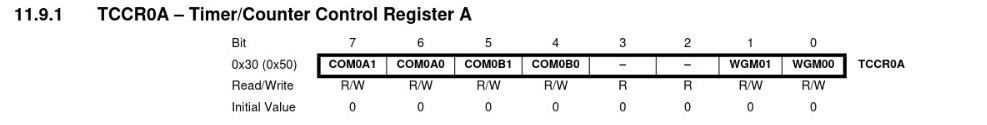
\includegraphics[scale=0.5]{images/TCCR0A_CL0.jpeg}
    \caption{Configuración del TCCR0A\cite{Atmel2011}.}
    \label{fig:enter-label}
\end{figure}
\begin{figure}[H]
    \centering
    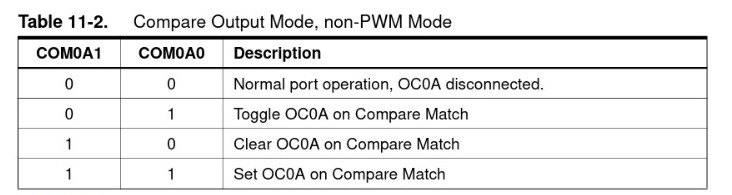
\includegraphics[scale=0.5]{images/COM0A.jpeg}
    \caption{Configuración del COMA0\cite{Atmel2011}.}
    \label{fig:enter-label}
\end{figure}
\begin{figure}[H]
    \centering
    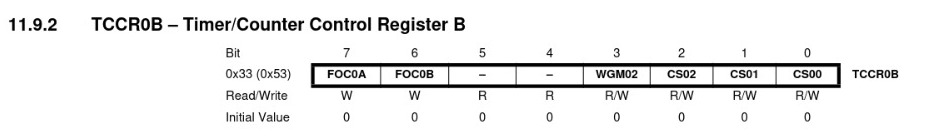
\includegraphics[scale=0.5]{images/TCCR0B.jpeg}
    \caption{Configuración del TCCR0B\cite{Atmel2011}.}
    \label{fig:enter-label}
\end{figure}
\begin{figure}[H]
    \centering
    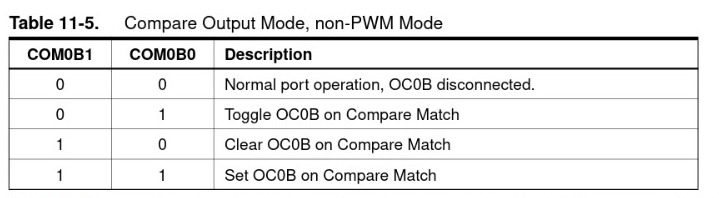
\includegraphics[scale=0.5]{images/COMB0.jpeg}
    \caption{Configuración del COMB0\cite{Atmel2011}.}
    \label{fig:enter-label}
\end{figure}
\subsubsection{Selección de la Fuente del Reloj}
Para el temporizador 0, la selección del reloj se controla con los bits CS0[2:0], y para el temporizador 1, con los bits CS1[2:0].






